\documentclass[8pt,a4paper]{article}

\usepackage{amsmath, amssymb, amsthm}
\usepackage{tikz}
\usepackage{mathtools}
\usepackage{multicol}
\usepackage[top=0.5cm,left=0.5cm,right=0.5cm,bottom=0.5cm]{geometry}
\usepackage{amsfonts}
\usepackage{etoolbox}
\usepackage{cancel}
\usepackage{yhmath}
\usepackage{color}
\usepackage{hyperref}
\usepackage{cancel}
\usepackage{graphicx}
\usepackage{caption}
\usepackage[overload]{empheq} % For braced-style systems of equations.

\newenvironment{Figure}
  {\par\medskip\noindent\minipage{\linewidth}}
  {\endminipage\par\medskip}

\newcommand{\RNum}[1]{\uppercase\expandafter{\romannumeral #1\relax}}

\definecolor{forestgreen(web)}{rgb}{0.13, 0.55, 0.13}
\definecolor{lavender(floral)}{rgb}{0.71, 0.49, 0.86}

\usepackage{nicefrac, xfrac}
%\usepackage{mathtools}
\newcommand{\abs}[1]{\left\lvert #1 \right\rvert}
\newcommand{\norm}[1]{\left\lVert #1 \right\rVert}
\newcommand{\sca}[1]{\left\langle #1 \right\rangle}

%\usepackage{xcolor}
\usepackage{titlesec}

%\usepackage{wasysym}
%\smiley{}

\usepackage{euscript} % accedi a Euler usando \EuScript{}
\newcommand{\pt}{\EuScript{P}}
\newcommand{\bt}{\EuScript{B}}
\renewcommand{\chi}{\EuScript{X}}
\newcommand{\ti}{\EuScript{T}}

% Bold
\renewcommand{\AA}{\mathbb A}
\newcommand{\BB}{\mathbb{B}}
\newcommand{\CC}{\mathbb{C}}
\newcommand{\DD}{\mathbb{D}}
\newcommand{\EE}{\mathbb{E}}
\newcommand{\FF}{\mathbb{F}}
\newcommand{\GG}{\mathbb{G}}
\newcommand{\HH}{\mathbb{H}}
\newcommand{\II}{\mathbb{I}}
\newcommand{\JJ}{\mathbb{J}}
\newcommand{\KK}{\mathbb{K}}
\newcommand{\LL}{\mathbb{L}}
\newcommand{\MM}{\mathbb{M}}
\newcommand{\NN}{\mathbb{N}}
\newcommand{\OO}{\mathbb{O}}
\newcommand{\PP}{\mathbb{P}}
\newcommand{\QQ}{\mathbb{Q}}
\newcommand{\RR}{\mathbb{R}}
\renewcommand{\SS}{\mathbb S}
\newcommand{\TT}{\mathbb{T}}
\newcommand{\UU}{\mathbb{U}}
\newcommand{\VV}{\mathbb{V}}
\newcommand{\WW}{\mathbb{W}}
\newcommand{\XX}{\mathbb{X}}
\newcommand{\YY}{\mathbb{Y}}
\newcommand{\ZZ}{\mathbb{Z}}

% Calligraphic
\newcommand{\Ac}{\mathcal{A}}
\newcommand{\Bc}{\mathcal{B}}
\newcommand{\Cc}{\mathcal{C}}
\newcommand{\Dc}{\mathcal{D}}
\newcommand{\Ec}{\mathcal{E}}
\newcommand{\Fc}{\mathcal{F}}
\newcommand{\Gc}{\mathcal{G}}
\newcommand{\Hc}{\mathcal{H}}
\newcommand{\Ic}{\mathcal{I}}
\newcommand{\Jc}{\mathcal{J}}
\newcommand{\Kc}{\mathcal{K}}
\newcommand{\Lc}{\mathcal{L}}
\newcommand{\Mc}{\mathcal{M}}
\newcommand{\Nc}{\mathcal{N}}
\newcommand{\Oc}{\mathcal{O}}
\newcommand{\Pc}{\mathcal{P}}
\newcommand{\Qc}{\mathcal{Q}}
\newcommand{\Rc}{\mathcal{R}}
\newcommand{\Sc}{\mathcal{S}}
\newcommand{\Tc}{\mathcal{T}}
\newcommand{\Uc}{\mathcal{U}}
\newcommand{\Vc}{\mathcal{V}}
\newcommand{\Wc}{\mathcal{W}}
\newcommand{\Xc}{\mathcal{X}}
\newcommand{\Yc}{\mathcal{Y}}
\newcommand{\Zc}{\mathcal{Z}}

% Bold Big Vector
\newcommand{\Av}{\mathbf{A}}
\newcommand{\Bv}{\mathbf{B}}
\newcommand{\Cv}{\mathbf{C}}
\newcommand{\Dv}{\mathbf{D}}
\newcommand{\Ev}{\mathbf{E}}
\newcommand{\Fv}{\mathbf{F}}
\newcommand{\Gv}{\mathbf{G}}
\newcommand{\Hv}{\mathbf{H}}
\newcommand{\Iv}{\mathbf{I}}
\newcommand{\Jv}{\mathbf{J}}
\newcommand{\Kv}{\mathbf{K}}
\newcommand{\Lv}{\mathbf{L}}
\newcommand{\Mv}{\mathbf{M}}
\newcommand{\Nv}{\mathbf{N}}
\newcommand{\Ov}{\mathbf{O}}
\newcommand{\Pv}{\mathbf{P}}
\newcommand{\Qv}{\mathbf{Q}}
\newcommand{\Rv}{\mathbf{R}}
\newcommand{\Sv}{\mathbf{S}}
\newcommand{\Tv}{\mathbf{T}}
\newcommand{\Uv}{\mathbf{U}}
\newcommand{\Vv}{\mathbf{V}}
\newcommand{\Wv}{\mathbf{W}}
\newcommand{\Xv}{\mathbf{X}}
\newcommand{\Yv}{\mathbf{Y}}
\newcommand{\Zv}{\mathbf{Z}}

% Bold Little Vector
\newcommand{\av}{\mathbf{a}}
\newcommand{\bv}{\mathbf{b}}
\newcommand{\cv}{\mathbf{c}}
\newcommand{\dv}{\mathbf{d}}
\newcommand{\ev}{\mathbf{e}}
\newcommand{\fv}{\mathbf{f}}
\newcommand{\gv}{\mathbf{g}}
\newcommand{\hv}{\mathbf{h}}
\newcommand{\iv}{\mathbf{i}}
\newcommand{\jv}{\mathbf{j}}
\newcommand{\kv}{\mathbf{k}}
\newcommand{\lv}{\mathbf{l}}
\newcommand{\mv}{\mathbf{m}}
\newcommand{\nv}{\mathbf{n}}
\newcommand{\ov}{\mathbf{o}}
\newcommand{\pv}{\mathbf{p}}
\newcommand{\qv}{\mathbf{q}}
\newcommand{\rv}{\mathbf{r}}
\newcommand{\sv}{\mathbf{s}}
\newcommand{\tv}{\mathbf{t}}
\newcommand{\uv}{\mathbf{u}}
\newcommand{\vv}{\mathbf{v}}
\newcommand{\wv}{\mathbf{w}}
\newcommand{\xv}{\mathbf{x}}
\newcommand{\yv}{\mathbf{y}}
\newcommand{\zv}{\mathbf{z}}

% Overarrow Little Vector
\newcommand{\bev}{\overrightarrow{\beta}}
\newcommand{\bbv}{\overrightarrow{b}}
\newcommand{\erv}{\overrightarrow{\varepsilon}}
\newcommand{\yev}{\overrightarrow{y}}

\renewcommand{\hat}{\widehat}

% differenziale
\newcommand{\dspace}{\,} % \, aggiunge un piccolo spazio
\newcommand{\de}{\mathrm{d}}
\newcommand{\dx}{\dspace \de x}
\newcommand{\dy}{\dspace \de y}
\newcommand{\dt}{\dspace \de t}
\newcommand{\dS}{\dspace \de S}
\newcommand{\ds}{\dspace \de s}
\newcommand{\dz}{\dspace \de z}
\newcommand{\dw}{\dspace \de w}
\newcommand{\du}{\dspace \de u}
\newcommand{\dvv}{\dspace \de v}
\newcommand{\db}{\dspace \de b}
\newcommand{\dteta}{\dspace \de \vartheta}
\newcommand{\dxi}{\dspace \de \xi}
\newcommand{\dxy}{\dspace \de x \de y}
\newcommand{\duv}{\dspace \de u \de v}
\newcommand{\dst}{\dspace \de s \de t}
\newcommand{\dP}{\dspace \de P}
\newcommand{\dPP}{\dspace \de \PP}
\newcommand{\dsig}{\dspace \de \sigma}
\newcommand{\dth}{\dspace \de \theta}
\newcommand{\deta}{\dspace \de \eta}
\newcommand{\dph}{\dspace \de \varphi}
\newcommand{\dxv}{\dspace \de \mathbf{x}}
\newcommand{\dSx}{\dspace \de \text{S}(x)}

\newcommand{\Bot}{\perp \!\!\! \perp} % indipendenza
\usepackage{dsfont} % per funzione indicatrice
\newcommand{\Ind}{\mathds{1}} % funzione indicatrice

\DeclareMathOperator{\Det}{det} % determinante
\DeclareMathOperator{\Img}{Im}
\DeclareMathOperator{\Ker}{Ker}
\DeclareMathOperator{\ArgMin}{ArgMin}
\DeclareMathOperator{\Div}{div}
\newcommand{\nabladot}{\nabla\!\!\cdot\!}
\DeclareMathOperator{\Lip}{Lip}

\renewcommand{\theta}{\vartheta}

% per far essere piccoli sum e prod
\makeatletter
\newcommand{\changeoperator}[1]{%
  \csletcs{#1@saved}{#1@}%
  \csdef{#1@}{\changed@operator{#1}}%
}
\newcommand{\changed@operator}[1]{%
  \mathop{%
    \mathchoice{\textstyle\csuse{#1@saved}}
               {\csuse{#1@saved}}
               {\csuse{#1@saved}}
               {\csuse{#1@saved}}%
  }%
}
\makeatother

\changeoperator{sum}
\changeoperator{prod}
 
 % Turn off header and footer
\pagestyle{empty}

% Redefine section commands to use less space
\makeatletter
\renewcommand{\section}{\@startsection{section}{1}{0mm}%
                                {-0.1ex plus -.5ex minus -.2ex}%
                                {1.5ex plus .2ex}%x
                                {\center\normalfont\large\bfseries}}
\renewcommand{\subsection}{\@startsection{subsection}{2}{0mm}%
                                {2ex plus 0ex minus 0ex}%
                                {1.5ex plus 0ex}%
                                {\normalfont\scriptsize\bfseries}}
\renewcommand{\subsubsection}{\@startsection{subsubsection}{3}{0mm}%
                                {-1ex plus -.5ex minus -.2ex}%
                                {1ex plus .2ex}%
                                {\normalfont\small\bfseries}}
\makeatother

\titlespacing\section{0pt}{0pt plus 0pt minus 0pt}{0pt plus 0pt minus 0pt}

% Don't print section numbers
\setcounter{secnumdepth}{0}

\setlength{\parindent}{0pt}
\setlength{\parskip}{0pt plus 0ex}

% -----------------------------------------------------------------------


\begin{document}

\raggedright
\footnotesize
\begin{multicols*}{3}

% multicol parameters
% These lengths are set only within the two main columns
%\setlength{\columnseprule}{0.25pt}
\setlength{\premulticols}{1pt}
\setlength{\postmulticols}{1pt}
\setlength{\multicolsep}{1pt}
\setlength{\columnsep}{2pt}

%!TEX root = ../main.tex

% =================================================

\section{\texorpdfstring{\color{red}Deformation and Motion}{}}

% =================================================

\begin{Figure}
    \center{
    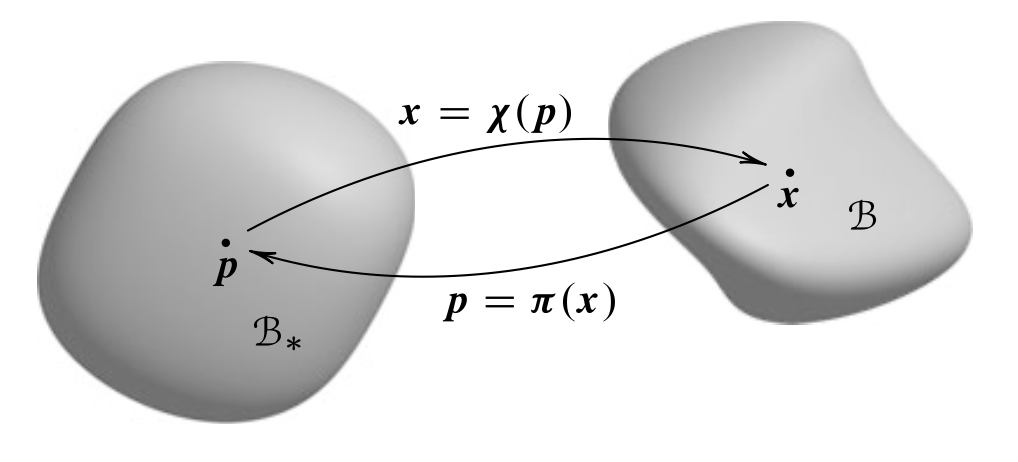
\includegraphics[width=0.8\linewidth]{images/def0}\ \ }
\end{Figure}

\textbf{Deformation gradient.} $F(p)=\nabla_{\!p}\chi$ such that
\begin{equation*}
\chi(q)=\chi(p)+F(p)[q-p]+o(q-p)
\end{equation*}

Fix origin and coordinate axes, $\de \underline{x}=F\,\de\underline{X}$ and component-wise it is
\begin{equation*}
F_{iK}=\frac{\partial x_i}{\partial X_K} 
\end{equation*}

Moreover, F can be seen as a linear trasformation
\begin{equation*}
F:T_{_X} \bt_*\to T_x \bt
\end{equation*}

\rule{0.31\textwidth}{0.2pt}
\smallskip

\textbf{Change of variables.} $\text{det}(F)=J>0$, then
\begin{align*}
\de V_x &= J\,\de V_{\!_X} \\
\underline{n}\,\de A_x &= JF^{\,\text{-}T}\underline{n}_*\,\de A_{_X}\quad(\text{Nanson})
\end{align*}

\rule{0.31\textwidth}{0.2pt}
\smallskip

\textbf{Homogeneous deformation.} When $F\in\text{Lin}^+$ is costant we have an homogeneous def. In addiction, if $q$ is a fixed point, then we have
\begin{equation*}
\chi(p)=q+F[p-q]
\end{equation*}
Moreover, if $F\equiv R\in \text{SO}(3)$ then we have a solid/rigid deformation.

\rule{0.31\textwidth}{0.2pt}
\smallskip

\textbf{Polar decomposition thm.} $\forall\,F\in\text{Lin}^+$ $\exists\,!$ $R\in\text{SO}(3)$, $U,V\in\!\text{Sym}^+$ st $F=RU=VR$.

\rule{0.31\textwidth}{0.2pt}
\smallskip

\textbf{Cauchy-Green tensors.} They are defined as
\begin{align*}
\text{left}\quad B&=FF^T=V^2 \\
\text{right}\quad C&=F^TF=U^2
\end{align*}

$B,C\in\text{Sym}^+$, $C$ \emph{lives} on $\bt_*$ and $B$ on $\bt$

\rule{0.31\textwidth}{0.2pt}
\smallskip

\textbf{Motion.} Simply, it's $\underline{x}=\chi(\underline{X},t)=\underline{x}(\underline{X},t)$, so
\begin{equation*}
F(\underline{X},t)=\nabla_{\!\! _X} \underline{x}(\underline{X},t)
\end{equation*}

\vspace{-1em}

\rule{0.31\textwidth}{0.2pt}
\smallskip

\textbf{Material and spatial gradient.} $\phi=\phi(\underline{x},t)$ spatial field, its spatial gradient is
\begin{equation*}
\nabla_{\!\!_x} \phi=\frac{\partial \phi}{\partial \underline{x}}
\end{equation*}

Instead, its material gradient is 
\begin{equation*}
\nabla_{\!\!_X} \phi_m=\frac{\partial \phi_m}{\partial \underline{X}}=\frac{\partial \phi_m}{\partial \underline{x}}\,\frac{\partial \underline{x}}{\partial \underline{X}}=\left( \nabla_{\!\!_x} \phi \right)_m \cdot F
\end{equation*}

formally, just $\boxed{\nabla_{\!\!_X} \phi=\nabla_{\!\!_x} \phi\cdot F}$

\rule{0.31\textwidth}{0.2pt}
\smallskip

\textbf{Velocity and acceleration.} They are
\begin{equation*}
\dot{\underline{x}}(\underline{X},t)=\frac{\partial\, \underline{x}(\underline{X},t)}{\partial t} \quad  \ddot{\underline{x}}(\underline{X},t)=\frac{\partial^2 \underline{x}(\underline{X},t)}{\partial t^2}
\end{equation*}

and $\underline{v},\underline{a}$ are the equivalent spatial representation.

\smallskip

The gradient of the material velocity is
\begin{equation*}
\nabla_{\!\!_{X}} \dot{\underline{x}}=\frac{\partial}{\partial \underline{X}} \frac{\partial\underline{x}}{\partial t}\overset{\scriptstyle\text{SW}}{=} \frac{\partial}{\partial t} \frac{\partial \underline{x}}{\partial \underline{X}}=\dot{F}
\end{equation*}

so formally, $\boxed{L:=\nabla_{\!\!x}\underline{v}=\dot{F}F^{\,\text{-}1}}$ 

\smallskip

By orthgonal decomposition for $2^{\text{nd}}$-rank tensor
\begin{equation*}
L=\frac{L+L^T}{2} +\frac{L-L^T}{2} =D+W
\end{equation*}

where $D\in\text{Sym}$ is the stretching tensor and $W\in\text{Skw}$ is the spin tensor.

\vspace{-0.5em}

\rule{0.31\textwidth}{0.2pt}
\smallskip

\textbf{Material and spatial time derivative.} $\phi$ spatial field, its spatial time derivative is
\begin{equation*}
\phi'=\frac{\partial \phi}{\partial t}
\end{equation*}

Instead, its material time derivative is 
\begin{equation*}
\left(\phi_m\right)^\cdot=\left(\phi'\right)_m+\left( \nabla_{\!\!_x} \phi \right)_m \cdot \dot{\underline{x}}
\end{equation*}

formally, just $\boxed{\dot{\phi}=\phi'+\nabla_{\!\!_x} \phi \cdot \underline{v}}$

\smallskip

Using this formula with $\phi\equiv \underline{v}$ we obtain
\begin{equation*}
\boxed{\underline{a}=\underline{v}'+ \left(\nabla_{\!\!_x}\underline{v} \right) \underline{v}}
\end{equation*}

\rule{0.31\textwidth}{1pt}












%!TEX root = ../main.tex

% =================================================

% \subsection{\color{red}Bho}

% =================================================
%!TEX root = ../main.tex

% =================================================

% \subsection{\color{red}Bho}

% =================================================
%!TEX root = ../main.tex

\vspace{-1em}

% =================================================
% =================================================

\section{\texorpdfstring{\color{red}Finite Elasticity}{}}

% =================================================
% =================================================

\textbf{Costitutive law.} $T=\hat{T}(F)$, where
\begin{equation*}
\hat{T}:\text{Lin}^+\to\text{Sym},\quad F\mapsto \hat{T}(F)=T
\end{equation*}

This forms a costitutive class (restriction), since given $\chi$ (i.e. given $F$), $T$ cannot not arbitrary. 

\rule{0.31\textwidth}{0.2pt}
\smallskip

\textbf{PFI.} From $T^*=\hat{T}(F^*)$ and $(\circledast)$ we deduce
\begin{equation*}
\boxed{Q\hat{T}(F)Q^T=\hat{T}(QF)\quad \forall\,Q\in\text{SO}(3)}
\end{equation*}

\textbf{Thm.} (PFI) $\Longleftrightarrow$ $\hat{T}(F)=R\,\widetilde{T}(U)R^T$

\rule{0.31\textwidth}{0.2pt}

% =================================================

\subsection{\texorpdfstring{\color{red}Perfect Fluids}{}}

% =================================================

\textbf{Costitutive law and simmetry group.} \\
$\qquad T=\hat{T}(F)\qquad G=\text{SL}(3)$

\rule{0.31\textwidth}{0.2pt}
\smallskip

\textbf{Thm (representation).} $T$ is a function of $\rho$ only and it is in the form $\boxed{T=\alpha(\rho)I}$

\rule{0.31\textwidth}{0.2pt}

% =================================================

\subsection{\texorpdfstring{\color{red}Isotropic Elastic Solids}{}}

% =================================================

\textbf{Costitutive law and simmetry group.} \\
$\qquad T=\hat{T}(F)\qquad G=\text{SO}(3)$

Thanks to polar decomposition thm
\vspace{-1em}

\begin{equation*}
\hat{T}(F)=\hat{T}(VR)\overset{G}{=}\hat{T}(VRQ)\overset{Q=R^T}{=}\hat{T}(V)
\end{equation*}
and $B=FF^T=V^2$ $\leadsto$ $T=\widetilde{T}(B)$

\rule{0.31\textwidth}{0.2pt}
\smallskip

\textbf{PFI.} From $T^*=\hat{T}(B^*)$ and $(\circledast)$ we deduce
\begin{equation*}
\boxed{Q\widetilde{T}(B)Q^T=\widetilde{T}(QBQ^T)\quad \forall\,Q\in\text{SO}(3)}
\end{equation*}

\rule{0.31\textwidth}{0.2pt}
\smallskip

\textbf{Thm (representation).} 
\begin{equation*}
\boxed{\widetilde{T}(B)=\beta_0I+\beta_1B+\beta_2B^2}
\end{equation*}

where $\beta_k=\beta_k(i_1(B),i_2(B),i_3(B))$ and $i_1=\text{tr}\,B$, $i_2=\nicefrac{\left(\text{tr}^2 B- \text{tr}\,B^2\right)}{2}$, $i_3=\text{det}\,B$.

\rule{0.31\textwidth}{0.2pt}
\smallskip

\textbf{Internal constraints.} They are $\varphi(F)=0$. The most important one gives incompressibility: $0=\varphi(F)=\text{det}\,F-1$ $\Longrightarrow$ $S_R=\alpha JF^{\,\text{-}T}$, $T_R=\alpha I$, thus
\begin{equation*}
\widetilde{T}(B)=\alpha I + \beta_1 (i_1,i_2)B+\beta_2(i_1,i_2)B^2
\end{equation*} 
because $i_3=\text{det}\,FF^T=\text{det}^2F=1$.

\rule{0.31\textwidth}{1pt}









%!TEX root = ../main.tex

% =================================================
% =================================================

\section{\texorpdfstring{\color{red}Viscoelasticity}{}}

% =================================================
% =================================================

\textbf{Costitutive law.} $T=\hat{T}(F,\dot{F})$ or, since $L=\dot{F}F^{\,\text{-}1}$ thus $\dot{F}=LF$, $T=\hat{T}(F,L)$.

\rule{0.31\textwidth}{0.2pt}
\smallskip

\textbf{Thm.} (PFI) $\Longrightarrow$ $T=\hat{T}(F,D)$

\rule{0.31\textwidth}{0.2pt}

% =================================================

\subsection{\texorpdfstring{\color{red}Viscoelastic Fluids}{}}

% =================================================

\textbf{Costitutive law and simmetry group.} \\
$\qquad T=\hat{T}(F,D)\qquad G=\text{SL}(3)$

Since $(FH)^\cdot(FH)^{\text{-}1}=L$ ($L$ not affected), the material simmetry implies only
\begin{equation*}
\hat{T}(F,D)=\hat{T}(FH,D)\quad\forall\,H\in\text{SL}(3)
\end{equation*}

Moreover, similar to perfect fluids, we have
\begin{equation*}
\boxed{\hat{T}(F,D)=\widetilde{T}(\rho,D)}
\end{equation*}

\rule{0.31\textwidth}{0.2pt}
\smallskip

\textbf{PFI.} $Q\widetilde{T}(\rho,D)Q^T=\widetilde{T}(\rho,QDQ^T)\quad\forall\,Q\in\text{SO}(3)$

\rule{0.31\textwidth}{0.2pt}
\smallskip

\textbf{Thm (representation).}
\begin{equation*}
\boxed{\widetilde{T}(\rho,D)=\alpha_0 I+\alpha_1D+\alpha_2D^2}
\end{equation*} 
where $\alpha_k=\alpha_k(\rho,i_1,i_2,i_3)$.

\smallskip

This is the most general relation, namely for \emph{non-newtonian compressible fluids}. Now, we can do two more things:

\smallskip

$ \bullet $ add the incrompressibility constraint
\begin{equation*}
\text{det}\,F=1\ \Leftrightarrow\ \text{div}\,\underline{v}=0 \ \Leftrightarrow\ \text{tr}\,D=0
\end{equation*}
$\ \ $ obtaining $T_R=-p(\underline{x})I$ thus
\begin{equation*}
T=-p(\underline{x})I+\alpha_1(\rho,i_2,i_3)D+\alpha_2(\rho,i_2,i_3)D^2
\end{equation*}
$\ \ $ because $i_1(D)=0$.

\smallskip

$ \bullet $ make it linear with $\alpha_2=0$ and $\alpha_1=2\mu$, \\
$\ \ $ obatining the representation for \emph{newtonian} \\
$\ \ $ \emph{incompressible fluids}
\begin{equation*}
T=T_R+T_{\text{vis}}=-p(\underline{x})I+2\mu D
\end{equation*}

$\ \ \ \ \diamond$ here we derive NS eqns
\begin{equation*}
\begin{cases}
\rho\,\dot{\underline{v}}=-\nabla p+\mu\,\Delta \underline{v}+ \underline{b} \\
\text{div}\,\underline{v}=0
\end{cases}
\end{equation*}

\rule{0.31\textwidth}{0.2pt}

% =================================================

\subsection{\texorpdfstring{\color{red}Isotropic Viscoelastic Solids}{}}

% =================================================

\textbf{Costitutive law and simmetry group.} \\
$\qquad T=\hat{T}(F,D)\qquad G=\text{SO}(3)$

Since $(FQ)^\cdot(FQ)^{\text{-}1}=L$ ($L$ not affected), the material simmetry implies only
\begin{equation*}
\hat{T}(F,D)=\hat{T}(FQ,D)\quad\forall\,Q\in\text{SO}(3)
\end{equation*}

Moreover, similar to elastic solids, we have
\begin{equation*}
\boxed{\hat{T}(F,D)=\widetilde{T}(B,D)}
\end{equation*}

\rule{0.31\textwidth}{0.2pt}
\smallskip

\textbf{PFI.} $Q\widetilde{T}(B,D)Q^T=\widetilde{T}(QBQ^T,QDQ^T)\quad\forall\,Q$

\rule{0.31\textwidth}{1pt}









%!TEX root = ../main.tex

\vspace{-1em}

% =================================================
% =================================================

\section{\texorpdfstring{\color{red}Hyperelasticity}{}}

% =================================================
% =================================================

\textbf{Def.} An elastic body is hyperelastic if there exists an \emph{elastic energy density per unit volume}
\begin{equation*}
\omega:\text{Lin}^+\to\RR\,, \qquad F\mapsto \omega(F)  
\end{equation*}
such that $\boxed{S=\nicefrac{\partial\omega}{\partial F}}$

\smallskip

$\leadsto\ S\cdot \dot{F}=\frac{\de\ \omega\big(F(\underline{x},t)\big)}{\de t}$, so $\Pi^{\,\text{int}}=-\frac{\de }{\de t}\int_{_{\pt_*}}\!\!\omega\ \de V_{_X}$

\rule{0.31\textwidth}{0.2pt}
\smallskip

\textbf{Thm (characterization of hyperelastic body).} $\exists\,\omega$ iff $ \oint_{t_0}^{t_1} S\cdot\dot{F}\dt=0$
for any mechanical process; this implies $\int S\cdot\dot{F}\dt$ depends only on the extremes.

\rule{0.31\textwidth}{0.2pt}
\smallskip

\textbf{Potential elastic energy.} $\Uc(\pt_*)=\int_{_{\pt_*}}\!\!\omega\ \de V_{_X}$

\smallskip

By $(\propto\!m)$, we know $\Pi^{\,\text{int}}=-\dot{\Uc}$, thus the kinetic energy thm becomes $\dot{T_k}+\dot{\Uc}=\Pi^{\,\text{ext}}$. Moreover, if external forces are conservative, i.e. $=\frac{\de \Vc}{\de t}$, then the thm simply is $\frac{\de}{\de t}\ (T_k+\Uc+\Vc)=0$.

\rule{0.31\textwidth}{0.2pt}
\smallskip 

One can rewrite using $\sigma(F)$ \emph{energy density per unit mass} st $\omega(F)=\rho_*\sigma(F)$, for istance
\vspace{-0.5em}
\begin{equation*}
\Uc=\int_{_{\pt_*}}\!\!\!\!\omega\ \de V_{_X}=\int_{_{\pt_*}}\!\!\!\!\rho_*\sigma\ \de V_{_X}=\int_{_{\pt_*}}\!\!\!\!\rho\,\sigma\ \de V_x
\end{equation*}
\vspace{-0.5em}
\rule{0.31\textwidth}{0.2pt}

\newcolumn

\textbf{PFI.} $\omega(F)=\omega(QF)$ $\forall Q\in\text{SO}(3)$

\smallskip

\textbf{Thm.} (PFI) $\Longleftrightarrow$ $T$ symmetric.

\rule{0.31\textwidth}{0.2pt}
\smallskip

Thanks to polar decomposition thm
\vspace{-1em}

\begin{equation*}
\omega(F)=\omega(QF)=\omega(QRU)\overset{Q=R^T}{=}\omega(U)
\end{equation*}
and $C=F^TF=U^2$ $\leadsto$ $\boxed{\omega=\hat{\omega}(C)}$

\smallskip

The advantage is that in this form the (PFI) is automatically satisfied, and in addiction
\begin{equation*}
\boxed{S=2F\,\textstyle\frac{\partial\,\hat{\omega}}{\partial C}}
\end{equation*}

and $T$ follows from $T=J^{\text{-}1}SF^T$.

\smallskip

With isotropic incompressible hyperel. materials
\begin{align*}
S&=-pF^{\,\text{-}T}+\textstyle\frac{\partial\,\omega}{\partial F} \\  
T&=-p\,I+\textstyle\frac{\partial\,\omega}{\partial F}\,F^T
\end{align*}


\rule{0.31\textwidth}{1pt}















%!TEX root = ../main.tex

\vspace{-1em}

% =================================================
% =================================================

\section{\texorpdfstring{\color{red}Termomechanics}{}}

% =================================================
% =================================================

\textbf{The first law of thermodynamics.} It represents a balance of energy
\begin{equation*}
\dot{T_k}(\pt_t)+\dot{\Uc}(\pt_t)=Q(\pt_t)+\Pi^{\,\text{ext}}(\pt_t)
\end{equation*}
Using the kinetic energy thm $\dot{T_k}=\Pi^{\,\text{ext}}+\Pi^{\,\text{int}}$
\begin{equation*}
\boxed{Q(\pt_t)=\dot{\Uc}(\pt_t)+\Pi^{\,\text{int}}(\pt_t)}
\end{equation*}
which, in its integral form is
\begin{equation*}
\int_{_{\pt_t}}\!\!\!\!\! \rho\,r\,\de V_x -\!\!\! \int_{_{\partial\pt_t}}\!\!\!\!\!\! \underline{q}\cdot \underline{n}\, \de A_x=\!\!\!\int_{_{\pt_t}}\!\!\!\!\!\rho\,\dot{e}\,\de V_x -\!\!\! \int_{_{\pt_t}}\!\!\!\!\! T\!\cdot\! D\,\de V_x
\end{equation*}

where $Q$ is the heat flowing into the body part given by the contribution of the \emph{heat source density} per unit mass $r(\underline{x},t)$ and the \emph{outgoing heat flux} $\underline{q}$ through the boundary, and $e$ is the \emph{internal energy density per unit mass}.

\smallskip

The local forms (using div. thm) are
\begin{equation*}
\boxed{
\begin{array}{c}
\rho\,r-\text{div}\,\underline{q}=\rho\,\dot{e}-T\cdot D \\
\rho_*r-\text{Div}\,\underline{q}_*=\rho_*\dot{e}-S\cdot \dot{F}
\end{array}
}
\tag{\RNum{1}}
\end{equation*}

where $\underline{q}_*=JF^{\,\text{-}1}\underline{q}$ is the heat flux in referential form which, as we did for Piola tensor, is st
\begin{equation*}
\int_{_{\partial\pt_t}}\!\!\!\! \underline{q}\cdot \underline{n}\ \de A_x= \int_{_{\partial\pt_*}}\!\!\!\! \underline{q}_*\!\!\cdot \underline{n}_*\ \de A_{_X}
\end{equation*}

\rule{0.31\textwidth}{0.2pt}
\smallskip

\textbf{The second law of thermodynamics.} It states the increase of entropy $\de S\geq\frac{\de Q}{T}$, due to the fact the entropy is $\de S=\frac{\de Q}{T}+\de S_{i}$ and the \emph{entropy production} $\de S_{i}\geq 0$.

\smallskip

\textbf{Rmk:} in reversible processes $\de S=\frac{\de Q}{T}$, instead in adiabatic processes $\de S=\de S_{i}\geq 0$. Moreover, one can rewrite the principle in the so called \emph{Clausius inequality} $\oint \frac{\de Q}{T} \leq 0$ .

\smallskip

By introducing $\vartheta(\underline{x},t)$ \emph{absolute temperature} and $\eta(\underline{x},t)$ \emph{entropy density per unit mass}, we write the integral form as
\begin{equation*}
\int_{_{\pt_t}}\!\!\!\!\! \rho\,\dot{\eta}\ \de V_x \geq
\int_{_{\pt_t}}\!\!\! \frac{\rho\,r}{\vartheta}\ \de V_x -\!\! 
\int_{_{\partial\pt_t}}\!\! \frac{\underline{q}}{\vartheta}\!\cdot \underline{n}\ \de A_x
\end{equation*}

or the local forms called \emph{Clausius-Duhem ineq.}
\begin{equation*}
\boxed{
{\renewcommand*{\arraystretch}{1.5}
\begin{array}{c}
\rho\,\theta\,\dot{\eta}\geq\rho\,r-\text{div}\,\underline{q}+\frac{1}{\vartheta}\,\underline{q}\cdot\nabla\vartheta \\
\rho_*\theta\,\dot{\eta}\geq\rho_*r-\text{Div}\,\underline{q}_*+\frac{1}{\vartheta}\,\underline{q}_*\!\cdot\nabla\vartheta
\end{array}}
} \tag{\RNum{2}}
\end{equation*}

where we used the div. thm and 
\begin{equation*}
\text{div}\left(\frac{\underline{q}}{\vartheta}\right)=\frac{1}{\vartheta}\,\text{div}\,\underline{q}-\frac{1}{\vartheta^2}\ \underline{q}\cdot\nabla \vartheta
\end{equation*}

Using (\RNum{1}) in (\RNum{2}) we get
\begin{equation*}
\boxed{
{\renewcommand*{\arraystretch}{1.5}
\begin{array}{c}
\rho\,\theta\,\dot{\eta}\geq\rho\,\dot{e}-T\cdot D+\frac{1}{\vartheta}\,\underline{q}\cdot\nabla\vartheta \\
\rho_*\theta\,\dot{\eta}\geq\rho_*\dot{e}-S\cdot\dot{F}+\frac{1}{\vartheta}\,\underline{q}_*\!\cdot\nabla\vartheta
\end{array}}
} \tag{\RNum{3}}
\end{equation*}

\rule{0.31\textwidth}{0.2pt}
\smallskip

\textbf{Dissipation inequality.} $\psi:=e-\theta\eta$ \emph{Helmholtz free energy density}, then (\RNum{3}) becomes
\begin{equation*}
\boxed{
\rho\,\dot{\psi}-T\cdot D+ \frac{1}{\vartheta}\ \underline{q}\!\cdot\!\nabla\vartheta+\rho\,\dot{\vartheta}\,\eta \leq 0
} \tag{\RNum{4}} 
\end{equation*}

\rule{0.31\textwidth}{1pt}














%!TEX root = ../main.tex

% =================================================
% =================================================

\section{\texorpdfstring{\color{red}Linear Elasticity}{}}

% =================================================
% =================================================

Here the focus is on the displacement $\underline{u}=\underline{x}-\underline{X}$. Since $\underline{x}(\underline{X},t)=\underline{X}+\underline{u}(\underline{X},t)$, the deformation gradient is $\boxed{F=I+\nabla_{\!\!_X} \underline{u}}$.  

\rule{0.31\textwidth}{0.2pt}
\smallskip

We consider $\underline{u}$ and $\nabla \underline{u}$ as small quantities, i.e. $\underline{u}=o(\Ec)=\nabla\underline{u}$, and we neglet terms of $o(\Ec^2)$.

\smallskip

In this framework, $C$ (also $B$) becomes
\vspace{-0.2em}
\begin{equation*}
\big(I+(\nabla \underline{u})^T\big) \big(I+\nabla \underline{u}\big)=I+2E+o(\Ec^2)
\end{equation*}
with $E:=\text{sym}\,\nabla\underline{u}$ \emph{infinitesimal strain tensor}.

\rule{0.31\textwidth}{0.2pt}
\smallskip

The elastic law $T=\hat{T}(F)$ becomes
\begin{equation*}
\hat{T}(I+\nabla\underline{u})=\underbracket[0.5pt]{\hat{T}(I)}_{:=T_0}+\underbracket[0.5pt]{D_F\hat{T}(I)}_{:=\CC}\big[\nabla\underline{u}\big]+o(\nabla\underline{u}) 
\end{equation*}
that is the \emph{infinitesimal elasticity law}.

\smallskip

However, we assume $T_0=0$ (i.e. no pre-stress), thus we have
\begin{equation*}
\boxed{T=\CC\big[\nabla\underline{u}\big]}
\end{equation*}

the \emph{linear elasticity law}.

\rule{0.31\textwidth}{0.2pt}
\smallskip

The \emph{linear elastic tensor} $\CC$ is
\begin{align*}
\CC:=D_F\hat{T}(I):\text{Lin}&\to\text{Sym} \\
\nabla\underline{u}&\mapsto \CC\big[\nabla\underline{u}\big]=T
\end{align*}

Since $T$ is symmetric i.e. $T_{ij}=T_{ji}$ then
\begin{equation*}
C_{ijhk}=\left.\frac{\partial T_{ij}}{\partial F_{hk}}\right|_{F_{hk}=I_{hk}} =C_{jihk}
\end{equation*}

Moreover, from (PFI) and $T_0=0$ one can deduce $\CC\big[\Omega\big]=0$ for every $\Omega\in\text{Skw}$, implying that
\begin{gather*}
\CC\big[\nabla\underline{u}\big]=\CC\big[\text{sym}\,\nabla\underline{u}\big]+\cancel{\CC\big[\text{skw}\,\nabla\underline{u}\big]}=\CC[E] \\
\leadsto\ \boxed{
\begin{aligned}
\CC:\text{Sym}&\to\text{Sym} \\
E&\mapsto T
\end{aligned}
\qquad C_{jihk}=C_{ijhk}=C_{ijkh}
}
\end{gather*}

\rule{0.31\textwidth}{0.2pt}
\smallskip

$T$ and $S$ are equivalent (negligible difference).

\rule{0.31\textwidth}{0.2pt}

% =================================================

\subsection{\texorpdfstring{\color{red}Isotropic Linear Elasticity}{}}

% =================================================

\textbf{Costitutive law and simmetry group.} \\
$\qquad T=\hat{T}(F)=\CC[E]\qquad G=\text{SO}(3)$

\rule{0.31\textwidth}{0.2pt}
\smallskip

\textbf{PFI.} $\boxed{Q\CC[E]Q^T=\CC[QEQ^T]\quad \forall\,Q\in\text{SO}(3)}$

\rule{0.31\textwidth}{0.2pt}
\smallskip

\textbf{Thm (representation).} 
\begin{equation*}
\boxed{\CC[E]=\lambda(\text{tr}\,E)I+2\mu E}
\end{equation*}
where $\lambda,\,\mu$ are the Lamé constants.

\rule{0.31\textwidth}{0.2pt}
\smallskip

\textbf{Balance equations.} From $\rho_*\ddot{\underline{x}}=\text{Div}\,S+\underline{b}_*$ we obtain the Navier equation
\begin{equation*}
\boxed{\rho_*\ddot{\underline{u}}=(\lambda+\mu)\nabla\big(\text{Div}\,\underline{u}\big)+\mu\,\Delta \underline{u}+\underline{b}_*}
\end{equation*}

\rule{0.31\textwidth}{1pt}










%!TEX root = ../main.tex

\vspace{-1em}

% =================================================
% =================================================

\section{\texorpdfstring{\color{red}Exercise Class Stuff}{}}

% =================================================
% =================================================

$F$-derivatives of $B$'s invariants:
\begin{equation*}
{\renewcommand*{\arraystretch}{2}
\begin{array}{l}
\text{D}_F\ J[U]=JF^{\,\text{-}T}\cdot U \\
\text{D}_F\ i_1(B)[U]=\text{tr}\big(UF^T+FU^T\big)=2F\cdot U \\
\text{D}_F\ i_2(B)[U]=2\Big(\underbracket[0.5pt]{\big(\text{tr}\,B\big)}_{i_1}F-BF  \Big)\cdot U \\
\text{D}_F\ \underbracket[0.5pt]{i_3(B)}_{J^2}[U]=2J\ \text{D}_F\ J[U]=2\underbracket[0.5pt]{J^2}_{i_3}F^{\,\text{-}T}\cdot U 
\end{array}}
\end{equation*}



\end{multicols*}

\end{document}